\documentclass[9pt]{beamer}

%~~~~~~~~~~~~~~~~~~~~~~~~~~~~~~~~~~~~~~~~~~~~~~~~~~~~~~~~~~~~~~~~~~~~~~~~~~~~~~
% Code
\newcommand{\code}[1]{\textcolor{white!25!black}{\texttt{#1}}}
%~~~~~~~~~~~~~~~~~~~~~~~~~~~~~~~~~~~~~~~~~~~~~~~~~~~~~~~~~~~~~~~~~~~~~~~~~~~~~~

%~~~~~~~~~~~~~~~~~~~~~~~~~~~~~~~~~~~~~~~~~~~~~~~~~~~~~~~~~~~~~~~~~~~~~~~~~~~~~~
% Include Figure
\usepackage{graphicx}
\usepackage{subcaption}
\usepackage{wrapfig}
%~~~~~~~~~~~~~~~~~~~~~~~~~~~~~~~~~~~~~~~~~~~~~~~~~~~~~~~~~~~~~~~~~~~~~~~~~~~~~~

%~~~~~~~~~~~~~~~~~~~~~~~~~~~~~~~~~~~~~~~~~~~~~~~~~~~~~~~~~~~~~~~~~~~~~~~~~~~~~~
% Use roboto Font (recommended)
\usepackage[sfdefault]{roboto}
\usepackage[utf8]{inputenc}
\usepackage[T1]{fontenc}
%~~~~~~~~~~~~~~~~~~~~~~~~~~~~~~~~~~~~~~~~~~~~~~~~~~~~~~~~~~~~~~~~~~~~~~~~~~~~~~

%~~~~~~~~~~~~~~~~~~~~~~~~~~~~~~~~~~~~~~~~~~~~~~~~~~~~~~~~~~~~~~~~~~~~~~~~~~~~~~
% Define where theme files are located. ('/styles')
\usepackage{styles/fluxmacros}
\usefolder{styles}
% Use Flux theme v0.1 beta
% Available style: asphalt, blue, red, green, gray
\usetheme[style=asphalt]{flux}
%~~~~~~~~~~~~~~~~~~~~~~~~~~~~~~~~~~~~~~~~~~~~~~~~~~~~~~~~~~~~~~~~~~~~~~~~~~~~~~

%~~~~~~~~~~~~~~~~~~~~~~~~~~~~~~~~~~~~~~~~~~~~~~~~~~~~~~~~~~~~~~~~~~~~~~~~~~~~~~
% Extra packages for the demo:
\usepackage{booktabs}
\usepackage{colortbl}
\usepackage{ragged2e}
\usepackage{schemabloc}
%~~~~~~~~~~~~~~~~~~~~~~~~~~~~~~~~~~~~~~~~~~~~~~~~~~~~~~~~~~~~~~~~~~~~~~~~~~~~~~
%~~~~~~~~~~~~~~~~~~~~~~~~~~~~~~~~~~~~~~~~~~~~~~~~~~~~~~~~~~~~~~~~~~~~~~~~~~~~~~
% Informations
\title{Análisis de Algoritmos II}
\subtitle{Un algoritmo de barrido de línea para agrupación espacial.\\
  \textbf{Profesores:}\\
  Jorge Urrutia Galicia\\
  Adriana Ramírez Vigueras\\
  Diego Jesús Favela Nava.}
\author{Aguilera Moreno Adrian.}
\institute{Facultad de Ciencias, UNAM}
\date{\today}
\titlegraphic{Imagenes/im1.png}
%~~~~~~~~~~~~~~~~~~~~~~~~~~~~~~~~~~~~~~~~~~~~~~~~~~~~~~~~~~~~~~~~~~~~~~~~~~~~~~

\begin{document}

% Generate title page
\titlepage

\begin{frame}
 \frametitle{Tabla de contenido.}
 \tableofcontents
\end{frame}
%%%%%%%%%%%%%%%%%%%%%%%%%%%%%%%%% Introducción:
\begin{frame}[plain]
  \begin{figure}
    \centering
    \begin{subfigure}[b]{0.6\textwidth}
      
\includegraphics[width=\textwidth]{./Imagenes/T1}
    \end{subfigure}
  \end{figure}
\end{frame}

\section{Introducción.}
%%%%%%%%%%%%%%%%%%% Pruebas
\begin{frame}{Introducción}{Historia...}
	\justifying
        Los \underline{relojes vectoriales} son un tipo de
        reloj lógico propuesto de manera independiente por
        \textit{Colin J. Fidge} y \textit{Friedemann Mattern}
        en 1988.
        
        \begin{center}
          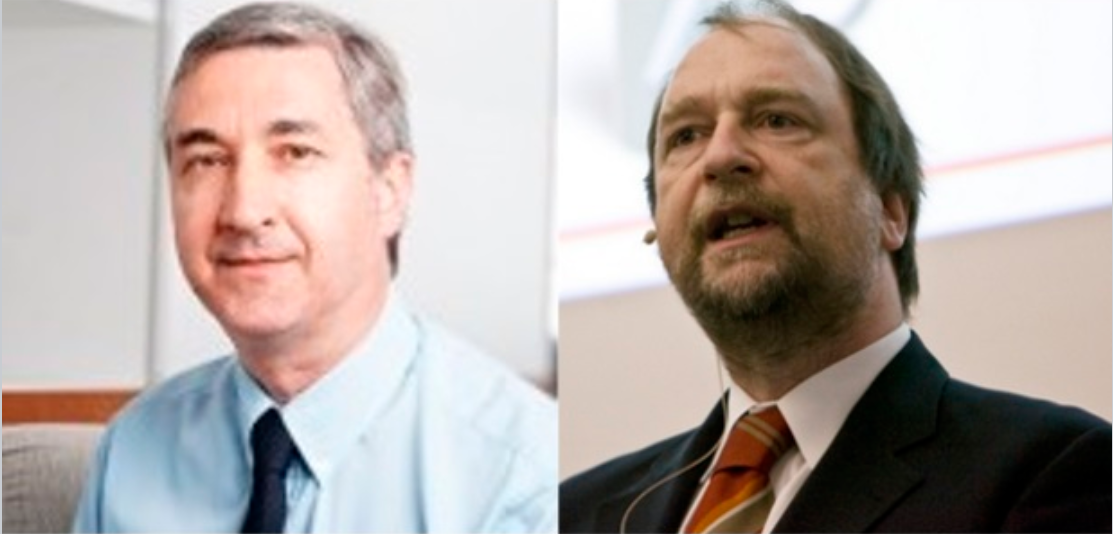
\includegraphics[height = 2cm]{./Imagenes/FidgeAndMattern.png}
        \end{center}
        
        Esta técnica consiste en un mapeo entre eventos en una
        historia distribuida y vectores enteros.
\end{frame}


\subsection{Categorías.}
%%%%%%%%%%%%%%%%%%%%%%%%%%%%%%%% Introducción:
\begin{frame}[fragile]{Categorías.}{}
  Existen dos categorías principales para realizar agrupamientos:
  \begin{enumerate}
  \item \textbf{Algoritmos de agrupamiento \textit{jerárquico}}.
    \begin{enumerate}
    \item Aglomerantes.
      
      Inicialmente cada objeto es un grupo, conforme transcurren las
      iteraciones los objetos se deben ir fucionando.
    \item Divisivos.
      
      Inicialmente todos los objetos son un solo grupo, conforma transcurren
      las iteraciones se van subdividiendo estos grupos.
    \end{enumerate}
  \item \textbf{Algoritmos de agrupamiento \textit{particional}}.
    
    Cada objeto se asocia con el centro de agrupamiento del más cercano.
  \end{enumerate}
  \begin{figure}
    \centering
    \begin{subfigure}[b]{0.4\textwidth}
      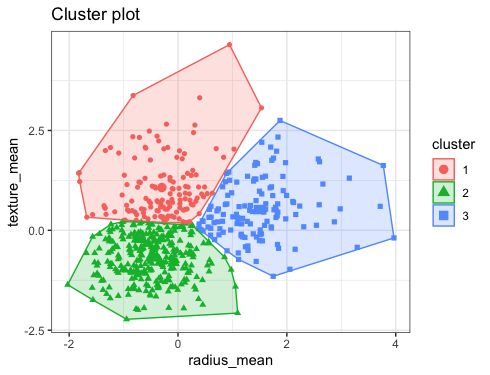
\includegraphics[width=\textwidth]{./Imagenes/kmeans.png}
      \caption*{Agrupamiento Particional.}
    \end{subfigure}
    \begin{subfigure}[b]{0.3\textwidth}
      \includegraphics[width=\textwidth]{./Imagenes/jerarquico.png}
      \caption*{Agrupamiento Jerárquico.}
    \end{subfigure}
  \end{figure}
\end{frame}


\subsection{Alternativas.}
%%%%%%%%%%%%%%%%%%%%%%%%%%%%%%%% Introducción:
\begin{frame}[fragile]{Alternativas.}{}
  \begin{wrapfigure}{r}{0.25\textwidth} %this figure will be at the right
    \centering
    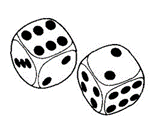
\includegraphics[width=0.25\textwidth]{./Imagenes/Aleatorios.png}
    \caption*{Aleatorios.}
  \end{wrapfigure}
  
  Algunas alternativas para agrupar son:
  \begin{enumerate}
  \item \textbf{Redes neuronales}.
  \item \textbf{k-means $+$ Algoritmos genéticos}.
  \item \textbf{Muestreos aleatorios}.
  \end{enumerate}

%  \begin{wrapfigure}{l}{0.25\textwidth}
%    \centering
%    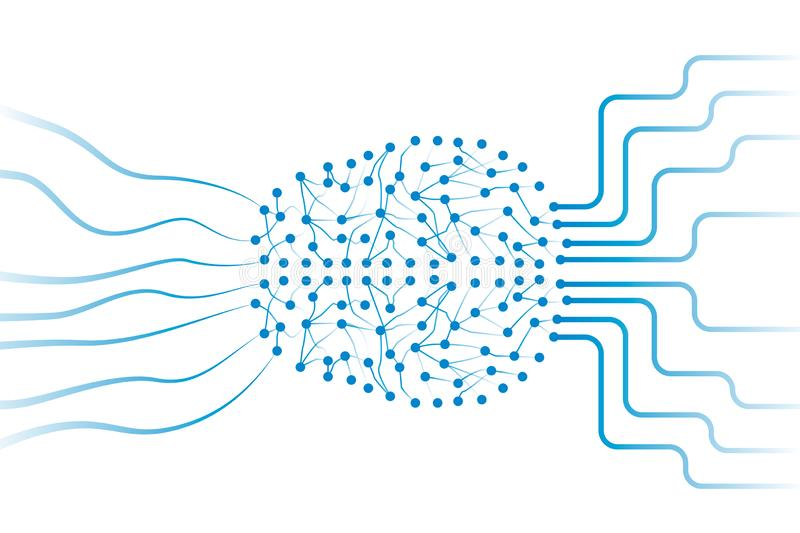
\includegraphics[width=0.25\textwidth]{Imagenes/RedNeuronal.jpg}
%  \end{wrapfigure}
  \begin{justify}  
    Algunas alternativas para agrupar basadas en el entrenamiento inteligente,
    búsquedas aleatorias (como las heurísticas), y uso de algoritmos genéticos
    (como las colonias de hormigas) son recurridas cuando no podemos garantizar
    un ``buen'' agrupamiento.
  \end{justify}
  
  \begin{figure}
    \centering
    \begin{subfigure}[b]{0.3\textwidth}
      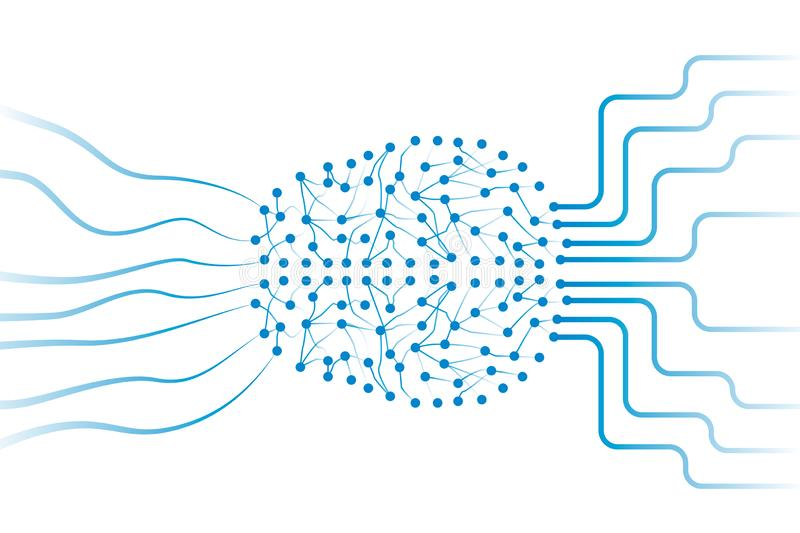
\includegraphics[width=\textwidth]{./Imagenes/RedNeuronal.jpg}
      \caption*{Redes Neuronales.}
    \end{subfigure}
    \begin{subfigure}[b]{0.3\textwidth}
      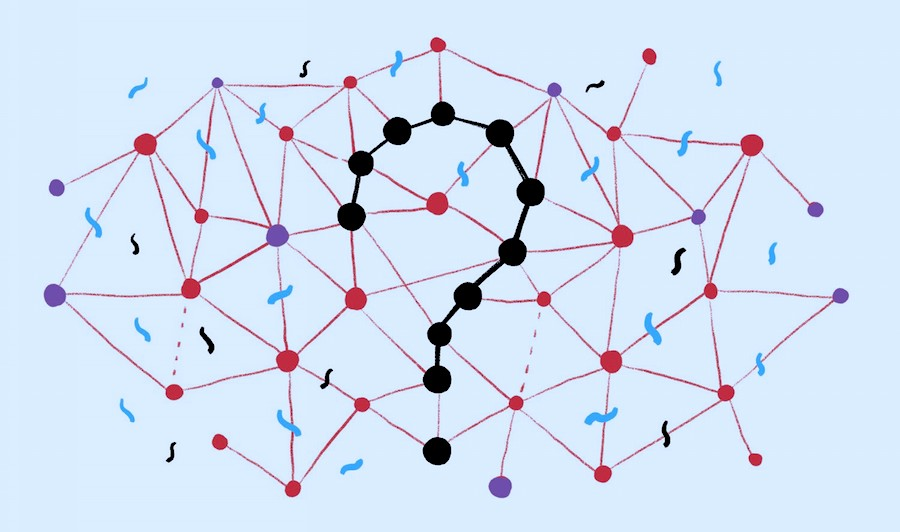
\includegraphics[width=\textwidth]{./Imagenes/Geneticos.jpeg}
      \caption*{K-means + Genéticos.}
    \end{subfigure}
  \end{figure}
\end{frame}


\subsection{Agrupación Espacial.}
%%%%%%%%%%%%%%%%%%%%%%%%%%%%%%%% Introducción:

\begin{frame}[fragile]{Agrupación Espacial:}{Propuestas I.}
  La agrupación espacial es un subconjunto espacial de agrupación. Este tipo
  de agrupamiento es relacionado, con frecuencia, a métodos gráficos.
  \begin{figure}
    \centering
    \begin{subfigure}[b]{0.3\textwidth}
      
\includegraphics[width=\textwidth]{./Imagenes/LeyGeo.png}
      %\caption*{Redes Neuronales.}
    \end{subfigure}
    \begin{subfigure}[b]{0.2\textwidth}
      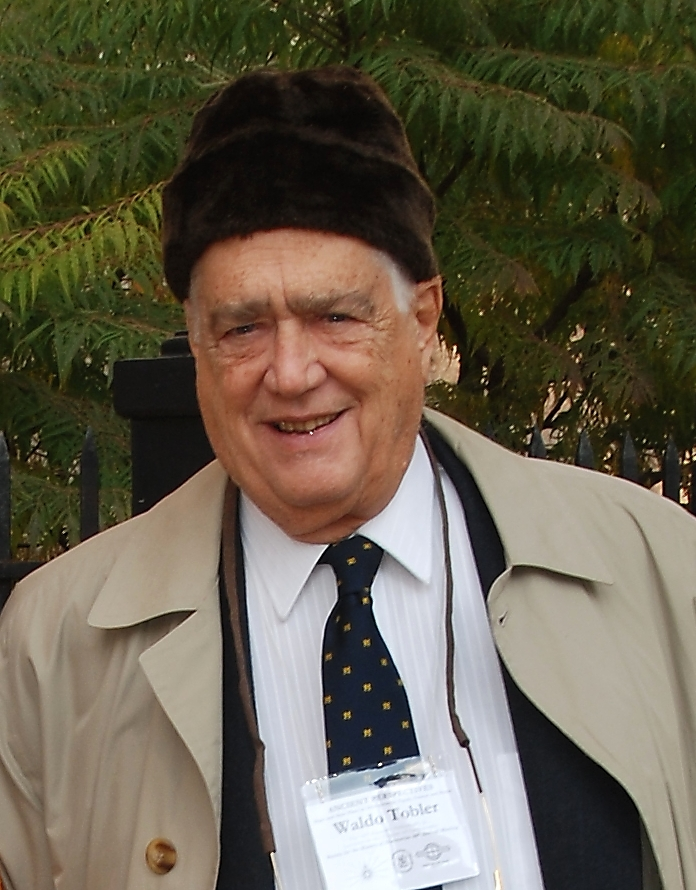
\includegraphics[width=\textwidth]{./Imagenes/Waldo_Tobler_2007.jpg}
      %\caption*{K-means + Genéticos.}
    \end{subfigure}
    \caption*{1era ley de la geografía.}
  \end{figure}
  \textbf{Propuestas:}
  \begin{itemize}
  \item Zahn sugiere trabajar con un gráfico completo (con vértices cada elemento en el espacio),
    construir el árbol de expansión mínima y eliminar los ``bordes'' más largos comparando las
    longitudes de los arcos con la longitud promedio, eliminando aquellos con longitud mayor al
    doble de la longitud promedio.
  \end{itemize}
\end{frame}

%%%%%%%%%%%%%%%%%%%%%%%%%%%%%%%% Introducción:

\begin{frame}[fragile]{Agrupación Espacial:}{Propuestas II.}
  \textbf{Propuestas:}
  \begin{itemize}
  \item Narendra sugiere el uso de diagramas de Voronoi para agrupar en
    tiempo $\mathcal{O}(n \log n)$. El problema de esta solución es que
    los algoritmos son dificiles de implementar.
  \item Kang usó triangulaciones de Delaunay y un diagrama dual de Voronoi.
    Después de construir la triangulación en $\mathcal{O}(n \log n)$, eliminamos
    las aristas con longitudes mayores a $d$.
  \item Yujian presentó un algoritmo de agrupamiento en subárboles máximos en
    distancia.
  \end{itemize}
  \textbf{¿Problemas? ...}
\end{frame}


%\def\beamer@mytheme@style{green}

%\subsection{Algoritmo.}
%%%%%%%%%%%%%%%%%%%% Especificación:
\begin{frame}{Reloj Vectorial:}{Algoritmo.}
  \justifying
  \textbf{Una primera aproximación.} Inicialmente
  todos los procesos disponen de un vector con
  entradas igual al número total de procesos, este
  vector debe estar inicializado en $0$ para cada
  entrada. A continuación se describe el algoritmo:
  \begin{itemize}
  \item[$\blacktriangleright$] Si $p_i$ produce un evento, entonces:
    \begin{enumerate}
    \item[(1)] $Vc_i[i] \leftarrow Vc_i[i] + 1$;
    \item[(2)] Produce un evento $e$ caracterizado por $Vc_i[1, \dotsm, n]$.
    \end{enumerate}
  \item[$\blacktriangleright$] Cuando $p_i$ envia un mensaje a $p_j$, entonces:
    \begin{enumerate}
    \item[(3)] $Vc_i[i] \leftarrow Vc_i[i] + 1$;
    \item[(4)] \code{send(\textlangle msj, $Vc_i$[1, $\dotsm$, n] \textrangle)} a $p_j$.
    \end{enumerate}
  \item[$\blacktriangleright$] Cuando $p_j$ recibe un mensaje, entonces:
    \begin{enumerate}
    \item[(3)] $Vc_j[j] \leftarrow Vc_j[j] + 1$;
    \item[(4)] $Vc_j[1, \dotsm, n] \leftarrow \forall_{k \in [1, \dotsm, n]}
      \code{max}(Vc_i[k], Vc_j[k])$.
    \end{enumerate}
  \end{itemize}
\end{frame}
 % Algoritmo.
%%%%%%%%%%%%%%%%%%%% Especificación:
\begin{frame}{Algoritmo:}{Propagación del tiempo vectorial.}
  \justifying
  \textbf{Notación:} Para, cualesquiera, dos vectores $Vc_1$
  y $Vc_2$ del tamaño $n$. Tenemos que
  \begin{itemize}
  \item[$\blacktriangleright$] $Vc_1 \leq Vc2 =_{def.}
    \left(\forall_{k \in \{1, \dotsm, n\}} : Vc_1[k] \leq Vc_2[k]\right)$;
  \item[$\blacktriangleright$] $Vc_1 < Vc2 =_{def.}
    \left(Vc_1[k] \leq Vc_2[k]\right) \land  \left(Vc_1[k] \not= Vc_2[k]\right)$;
  \item[$\blacktriangleright$] $Vc_1 || Vc_2 =_{def} \neg (Vc_1 \leq Vc_2) \land
    \neg (Vc_2 \leq Vc_1)$.
  \end{itemize}
  \begin{figure}
    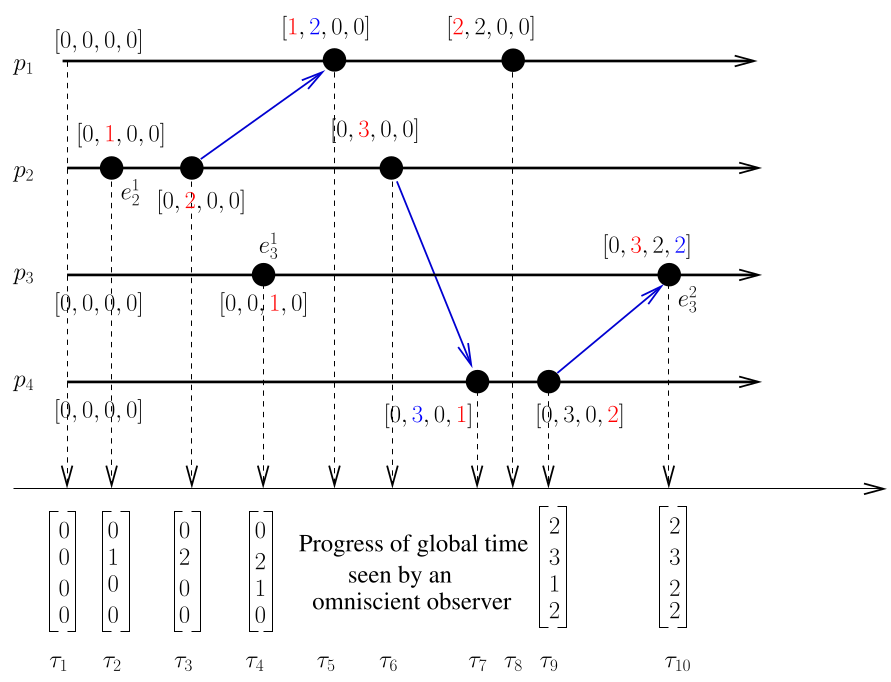
\includegraphics[height = 4.5cm]{./Imagenes/RelojVectorialCompuesto.png}
    \caption{Ejemplo de propagación en un reloj Vectorial.}
  \end{figure}
\end{frame}
 % Propagación del tiempo vectorial.
%%%%%%%%%%%%%%%%%%%% Especificación:
\begin{frame}[fragile]{Algoritmo:}{Propiedades.}
  \justifying
  \textbf{Def.} Sea $e.Vc$ el vector asociado al evento $e$.\\[0.3cm]
  
  \textbf{Teo 1.} Por el algoritmo mencionado tenemos que, para cualesquiera
  $e_1$ y $e_2$ distintos tenemos que
  \begin{enumerate}
  \item[$a$)] $\left(e_1 \rightarrow e_2\right) \Leftrightarrow \left(e_1.Vc < e_2.Vc\right)$;
  \item[$b$)] $\left(e_1 || e_2\right) \Leftrightarrow \left(e_1.Vc || e_2.Vc\right)$.
  \end{enumerate}
  
  \textbf{Cor 1.} Dadas dos caracterizaciones a eventos (fechas), determinar si estos
  eventos están relacionados o no, puede requerir hasta $n$ comparaciones de enteros.
  \\[0.3cm]
  
  \textbf{Teo 2.} Sean dos eventos $e_1$ y $e_2$ con tuplas $\langle e_1.Vc, i \rangle$
  y $\langle e_2.Vc, j\rangle$ de manera respectiva y $i \not= j$. Entonces
  \begin{enumerate}
  \item[$a$)] $\left(e_1 \rightarrow e_2\right) \Leftrightarrow
    \left(e_1.Vc[i] \leq e_2.Vc[i]\right)$;
  \item[$b$)] $\left(e_1 || e_2\right) \Leftrightarrow
    \left((e_1.Vc[i] > e_2.Vc[i]) \land (e_2.Vc[j] > e_1.Vc[j])\right)$.
  \end{enumerate}
\end{frame}
 % Propiedades.
%%%%%%%%%%%%%%%%%%%% Especificación:
\begin{frame}{Algoritmo:}{Reducción de costo en la comparación de dos vectores.}
  \justifying
  \textbf{Mejora en la complejidad en tiempo.} Hasta el momento la complejidad
  en tiempo para combinar $2$ eventos nos toma $\mathcal{O}(n)$, con $n$ el
  número de procesos en el sistema.\\[0.3cm]

  Por el \textit{Teo. 2}, sabemos que basta con verificar dos entradas para
  saber como es un evento respecto al otro. Así, basta comparar dos entradas
  para combinar la caracterización de $2$ eventos esto nos toma $\mathcal{O}(1)$.
\end{frame}
 % Reducción de costo en la comparación de dos vectores.
%%%%%%%%%%%%%%%%%%%% Especificación:
\begin{frame}[fragile]{Algoritmo:}{Relación del tiempo vectorial y estados globales.}
  \justifying
  Consideremos 
\end{frame}
 % Relación del tiempo vectorial y estados globales.

%\subsection{Desventajas.}
%%%%%%%%%%%%%%%%%%%% Especificación:
\begin{frame}[fragile]{Relojes Vectoriales:}{Desventajas.}
  Esta mejora a los relojes lógicos de Lamport tiene un problema
  de implementación, que en un momento será más evidente. 

  \setblockstyle{native} % Default behavior, optional line.
  \begin{center}
    \begin{minipage}[b]{0.5\textwidth}
      \begin{exampleblock}{Desventaja}
        Esta desventaja es que cada proceso tiene que cargar con espacio
        igual al número de procesos en el sistema y cada intercambio
        entre eventos es de este tamaño.
      \end{exampleblock}    
    \end{minipage}
  \end{center}
\end{frame}
  % Desventajas.

% The [plain] causes the headlines, footlines, and sidebars
% to be suppressed. Useful for showing large pictures

% TODO. Sin implementar.
%%%%%%%%%%%%%%%%%%%%%%%%%%%%%%%%% Aplicación:
\begin{frame}[plain]
  \begin{figure}
    \centering
    \begin{subfigure}[b]{0.6\textwidth}
      
\includegraphics[width=\textwidth]{./Imagenes/T2}
    \end{subfigure}
  \end{figure}
\end{frame}

%\section{Aplicaciones.}
%\subsection{El caso DynamoDB.}
%\begin{frame}[fragile]{Aplicación:}{DynamoDB}
    \justifying

Es un servicio de base de datos noSQL ofrecido por Amazon como parte de\\
Amazon Web Services.

\begin{center}
    
\includegraphics[scale=0.15]{D.jpg}
    \end{center}

De manera general lo utilizan para poder controlar el orden de los registros
de multiversión.

\end{frame}

%\begin{frame}[fragile]{Aplicación:}{DynamoDB}
    \justifying

    Problema:
    Alta disponibilidad para escrituras

    Técnica:
    Relojes vectoriales con reconciliación durante las lecturas.

    Ventaja:
    El tamaño de la versión está desvinculado de las tasas de actualización.

\end{frame}

%\begin{frame}[fragile]{Aplicación:}{DynamoDB}
    \justifying

    Dynamo utiliza relojes vectoriales para mantener el control de versiones del
    objeto en varias réplicas. Un reloj vectorial es efectivamente una lista de
    pares (nodo, contador). Un reloj vectorial está asociado con cada versión de
    cada objeto.

    \begin{center}
        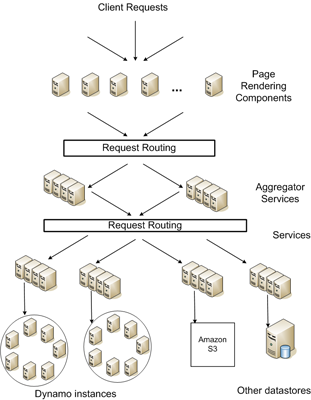
\includegraphics[scale=0.4]{D2.png}
        \end{center}

\end{frame}

%\begin{frame}[fragile]{Aplicación:}{DynamoDB}
    \justifying

    {\bf Para que los utiliza:}\\[0.3cm]

    Para capturar la causalidad entre diferentes versiones del mismo objeto.\\[0.3cm]

    Un reloj vectorial está asociado con cada versión de cada objeto. Uno puede
    determinar si dos versiones de un objeto están en ramas paralelas o tienen un
    orden causal, examinando sus relojes vectoriales.\\[0.3cm]

    Si los contadores del reloj del primer objeto son menores o iguales que todos
    los nodos del segundo reloj, entonces el primero es un ancestro del segundo y
    puede olvidarse. De lo contrario, se considera que los dos cambios están en
    conflicto y requieren reconciliación.

\end{frame}

%\begin{frame}[fragile]{Aplicación:}{DynamoDB}
    \justifying

    {\bf Como lo hace:}\\[0.3cm]

    Cuando un cliente desea actualizar un objeto, debe especificar qué versión está
    actualizando. Esto se hace pasando el contexto que obtuvo de una operación de
    lectura anterior, que contiene la información del reloj vectorial.\\[0.3cm]

    Al procesar una solicitud de lectura, si Dynamo tiene acceso a varias ramas que
    no se pueden reconciliar sintácticamente, devolverá todos los objetos en las
    hojas, con la información de versión correspondiente en el contexto. Se considera
    que una actualización que usa este contexto ha reconciliado las versiones
    divergentes y las ramas se contraen en una sola versión nueva.

\end{frame}

%\begin{frame}[fragile]{Aplicación:}{DynamoDB}
    \justifying

    {\bf Ejemplo:}\\[0.3cm]

%%%Anexar imagen Dynamo1
\begin{center}
    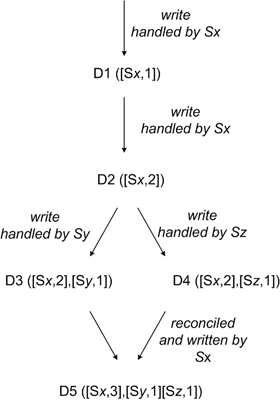
\includegraphics[scale=0.5]{D1.png}
    \end{center}
\end{frame}

%\begin{frame}[fragile]{Aplicación:}{DynamoDB}
    \justifying

    {\bf Ejemplo:}\\[0.3cm]

\begin{itemize}

\item Se tiene un nodo Sx, que maneja la escritura de esta clave aumenta su número
de secuencia y lo usa para crear el reloj vectorial de los datos.

\item Se tiene un objeto D1 y su reloj asociado [(Sx, 1)]. Este cliente lo actualiza
Supongamos que el mismo nodo también maneja esta solicitud.

\item Ahora el sistema tendra un objeto D2 y su reloj asociado [(Sx, 2)].

\item D2 desciende de D1, y por lo tanto sobrescribe D1

\item Supongamos que el mismo cliente actualiza el objeto nuevamente y un
servidor diferente maneja la solicitud (por ejemplo Sy).

\item Se tiene datos D3 y su reloj asociado [(Sx, 2), (Sy, 1)].


\end{itemize}


\end{frame}

%\begin{frame}[fragile]{Aplicación:}{DynamoDB}
    \justifying

    {\bf Ejemplo:}\\[0.3cm]

    Ahora supongamos que un cliente diferente lee D2 y luego intenta actualizarlo,
    y otro nodo realiza la escritura (por ejemplo, Sz).

\begin{itemize}
\item El sistema va a tener a D4 (descendiente de D2) cuya versión de reloj es
[(Sx, 2), (Sz, 1)].

\item Un nodo que es consciente de D3 y recibe D4 encontrará que no existe una
relación causal entre ellos. Esto quiere decir que hay cambios en D3 y D4 que
no se reflejan entre sí.

\item Ambas versiones de los datos deben conservarse y presentarse a un cliente
(después de una lectura) para la reconciliación semántica.

\end{itemize}

\end{frame}

%\begin{frame}[fragile]{Aplicación:}{DynamoDB}
    \justifying

    {\bf Ejemplo:}\\[0.3cm]

    Ahora supongamos que algún cliente lee tanto D3 como D4 (el contexto nos dirá
    que la lectura encontró ambos valores)\\[0.3cm]

    {\bf Nota:} El contexto de la lectura es un resumen de los relojes de D3 y D4, a
    saber, [(Sx, 2), (Sy, 1), (Sz, 1)]. Entonces

\begin{itemize}
\item Si el cliente realiza la reconciliación y el nodo Sx coordina la escritura,
Sx actualizará su número de secuencia en el reloj.

\item Finalmente el nuevo dato D5 tendrá el siguiente reloj:
[(Sx, 3), (Sy, 1), (Sz, 1)].
\end{itemize}

\end{frame}

%\begin{frame}[fragile]{Aplicación:}{DynamoDB}
    \justifying

{\bf Posible desvantaja de esto es:}

Es que el tamaño de los relojes vectoriales puede crecer si muchos servidores
coordinan las escrituras en un objeto.\\[0.3cm]

{\bf Lo provoca:}\\[0.3cm]
En caso de particiones de red o fallas de múltiples
servidores, las solicitudes de escritura pueden ser manejadas por nodos que no
están en los primeros N nodos en la lista de preferencias\\[0.3cm]

{\bf Para evitar lo anterior:}\\[0.3cm]
Se emplea el siguiente esquema de truncamiento de reloj:
Junto con cada par (nodo, contador), Dynamo almacena una marca de tiempo que
indica la última vez que el nodo actualizó el elemento de datos. Cuando el
número de pares en el reloj vectorial alcanza un umbral, el par más antiguo se
elimina del reloj.
\end{frame}

%\begin{frame}[fragile]{Aplicación:}{DynamoDB}
    \justifying

    Este problema no ha surgido en la producción y, por lo tanto, este problema
    no se ha investigado a fondo.

    \begin{center}
        
\includegraphics[scale=0.3]{D3.jpg}
        \end{center}


\end{frame}

%\begin{frame}[fragile]{Aplicación:}{DynamoDB}
    \justifying

    {\bf Algunas empresas que lo utilizan:}\\[0.3cm]

\begin{itemize}
\item Lyft
\item Airbnb
\item Redfin
\item Samsung
\item Toyota
\item Capital One
\end{itemize}

\end{frame}

%%%%%%%%%%%%%%%%% Nat:
% Solo es el orden, cambia lo que quieras (títulos). Perdón.
%----------------------------------------------------------
%\subsection{Relojes vectoriales dinámicos.}   %%%%%%%%%%%%%%%%%%%% Nat, aquí.  %%%%%%%%%%%%%%%%%%%%
%%%%%%%%%%%%%%%%%%%% Especificación:
\begin{frame}[fragile]{Aplicación:}{Relojes vectoriales dinamicos}
    \justifying
    A menudo el número de procesos participando en un computo distribuido no es constante, por lo que los relojes debe ser capaces de crecer.
    
    %Para alcanzar esta flexibilidad el vector de reloj es una matriz de dos columnas, variable en su número de filas, que proporciona un mapeo simple de la ID de un proceso al valor de reloj asociado (escalar).

    El tamaño del vector está limitado por dos veces el número de procesos de los que el proceso de mantenimiento ha recibido (directa o indirectamente) valores de reloj.
    
    Cada proceso $p_i$ mantiene su propio reloj logico $C_i$ el cual es una matriz de dos columnas, variable en su número de filas, donde $C_i(e_i^x)[k,2]$, en $e_i$ almacena el valor del último reloj vectorial conocido por $p_i$ del proceso cuyo ID está en $C_i(e_i^x)[k,1]$ 

    \begin{figure}
        \centering
        \begin{subfigure}[b]{0.5\textwidth}
            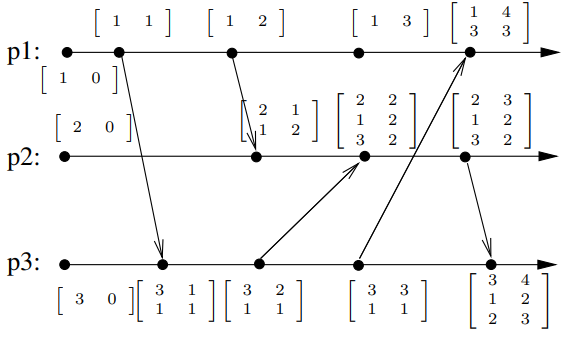
\includegraphics[width=\textwidth]{./rvd01.png}
            \caption{Reloj vectorial dinamico.}\label{fig:Deteccion.}
            \label{fig:Relojes vectoriales dinamicos}
        \end{subfigure}
    \end{figure}    
\end{frame}
%%%%%%%%%%%%%%%%%%%% Especificación:
\begin{frame}[fragile]{Aplicación:}{Relojes vectoriales dinamicos}
    \justifying

    Inicialmente, el reloj consiste de una sola fila con $C_i(e_i^0)[1,1]=i$ y $C_i(e_i^0)[1,2]=0$

    \textbf{Las reglas para actualizar son las siguientes:} 
    
    \begin{enumerate}
        \item Al recibir el $m$ de $e_i^x$, entonces $\forall l$ que no exceda el número de filas en $C_j(e_j^y)$: $C_j(e_j^y) = max\{C_i(e_i^{x-1})[k,2], C_j(e_j^y)[1,2]\}$, donde $C_j(e_j^y)$ la matriz de reloj del evento enviado en el proceso $J$ que envio $m$ al proceso $i$, y $C_j(e_j^y)[l,1]=C_i(e_i^x)[k,1]$
        
        \item Si no existe $k$ tal que $C_i(e_i^x)[k,1] = C_j(e_j^y)[l,1]$ para cualquier l, entonces una nueva fila es añadida a $C_i(e_i^x)$ con $C_i(e_i^x)[k,1] = C_j(e_j^y)[l,1]$ y $C_i(e_i^x)[k,2] = C_j(e_j^y)[l,2]$
        
        \item Si $e_i^x$ es cualquier evento, entonces el proceso incrementa su reloj vectorial: $C_i(e_i^x)[1,2] = C_i(e_i^{x-1})[1,2]+1$

  \end{enumerate}
\end{frame}
%%%%%%%%%%%%%%%%%%%% Especificación:
\begin{frame}[fragile]{Aplicación:}{Relojes vectoriales dinamicos}
    \justifying
    
    De manera similar podemos hacer una prueba de dependencia causal de la forma:
    $e_i^x \implies e_j^y)$ si y solo si $\exists k,l$:
    $$C_i(e_i^x)[k,1] = C_j(e_j^y)[l,1] = i$$
    y 
    $$C_i(e_i^x)[k,2] \leq C_j(e_j^y)[l,2]$$

    Y de concurrencia
    $e_i^x || e_j^y$ si y solo si
    $$C_j(e_j^y) \nleq C_i(e_i^x)$$
    y
    $$C_i(e_i^x) \nleq C_j(e_j^y)$$
\end{frame}
%\subsection{Seguimiento del predecesor inmediato (IPT).}
%%%%%%%%%%%%%%%%%%%% Especificación:
\begin{frame}[fragile]{Vector Clocks in Action:}{Immediate Precessors}
    \justifying
    \textbf{Evento relevante} En algún nivel de abstracción, sólo un subconjunto de los eventos son relevantes. Por ejemplo, en algunas aplicaciones sólo la modificación de algunas variables locales, o el procesamiento de ciertos mensajes especificos son relevantes.
    
    Dado un computo distribuido
    $\widehat{H}=(H,\xrightarrow[]{ev})$, sea $R\subset H$ los eventos relevantes.

    \textbf{Definición. Relación causal de Precedencia}, denotada como $\xrightarrow[]{re}$:
    $$\forall e_1,e_2 \in R : (e_1 \xrightarrow[]{re} e_2) \iff (e_2 \xrightarrow[]{ev} e_1)$$

    Esta relación es la proyección de $\xrightarrow[]{ev}$ sobre los elementos de R.
    
    %Sin perder generalidad, consideramos que $R$ consiste solo de eventos internos. Los eventos de comunicación son eventos de bajo nivel que, sin ser relevantes en sí mismos, participan en el establecimiento de una precedencia causal sobre eventos relevantes. Si un evento de comunicación necesita ser observado como relevante explícitamente, un evento interno asociado puede ser creado antes o despues de este. 

    Sean $e_1,e_2 \in R$. Si $e_1$ es \textbf{predecesor inmediato de} $e_2$ entonces:
    $$(e_1 \xrightarrow[]{re} e_2) \wedge (\nexists e \in : (e_1 \xrightarrow[]{re} e) \wedge (e \xrightarrow[]{re}e_2))$$

\end{frame}
%%%%%%%%%%%%%%%%%%%% Especificación:
\begin{frame}[fragile]{Vector Clocks in Action:}{Immediate Precessors}
    \justifying
    \begin{figure}
        \centering
        ~ %add desired spacing between images, e. g. ~, \quad, \qquad, \hfill etc. 
        %(or a blank line to force the subfigure onto a new line)
        \begin{subfigure}[b]{0.5\textwidth}
            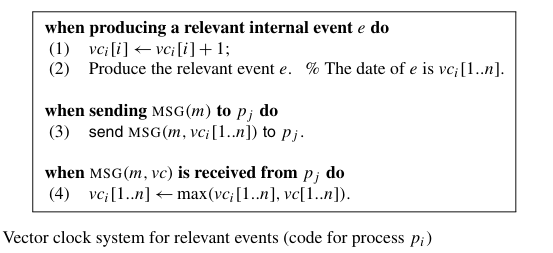
\includegraphics[scale=0.6]{Imagenes/eventosRelevantes02.png}
            \label{fig:ejemplo2}
        \end{subfigure}
        \begin{subfigure}[b]{0.5\textwidth}
            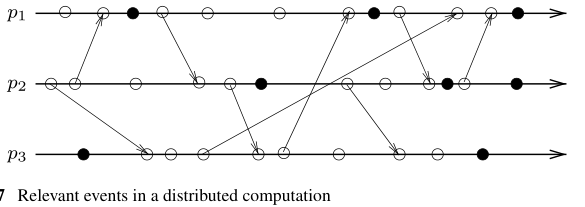
\includegraphics[scale=0.6]{Imagenes/eventosRelevantes01.png}
            \label{fig:ejemplo1}
        \end{subfigure}
        ~ %add desired spacing between images, e. g. ~, \quad, \qquad, \hfill etc. 
          %(or a blank line to force the subfigure onto a new line)
    \end{figure}
\end{frame}
%%%%%%%%%%%%%%%%%%%% Especificación:
\begin{frame}[fragile]{Vector Clocks in Action:}{Immediate Precessors}
    \justifying
    \textbf{El problema del seguimiento del predecesor inmediato (Immediate predecessor tracking IPT)} 
    Consiste en asociar a cada evento relevante el conjunto de eventos relevantes que son sus predecesores inmediatos.

    Además, esto se ha hecho sobre la marcha y sin añadir mensajes de control.
    
    La determinación de los predecesores inmediatos consiste en calcular la reducción transitiva (o diagrama de Hasse) del orden parcial $\widehat{R}=(R,\xrightarrow[]{re})$. 

    \justifying
    \begin{figure}
        \begin{subfigure}[b]{\textwidth}
            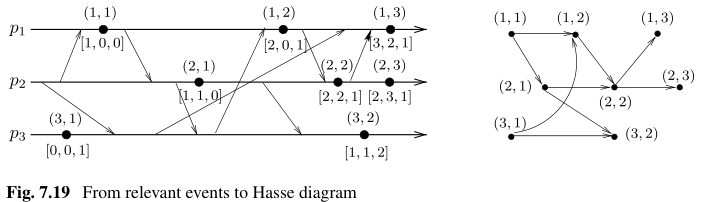
\includegraphics[scale=0.7]{Imagenes/eventosRelevantes03.png}
            \label{fig:ejemplo2}
        \end{subfigure}
    \end{figure}

\end{frame}
%%%%%%%%%%%%%%%%%%%% Especificación:
\begin{frame}[fragile]{Vector Clocks in Action:}{Immediate Precessors}
    \justifying
    \textbf{Un algoritmo que resuelve el problema IPT: variables locales}
    %El k-ésimo evento relevante en el proceso pk se identifica inequívocamente por el par (k,vck), donde vck es el valor de vck[k] cuando pk ha producido este evento.
    \begin{figure}
        \centering
        \begin{subfigure}[b]{\textwidth}
            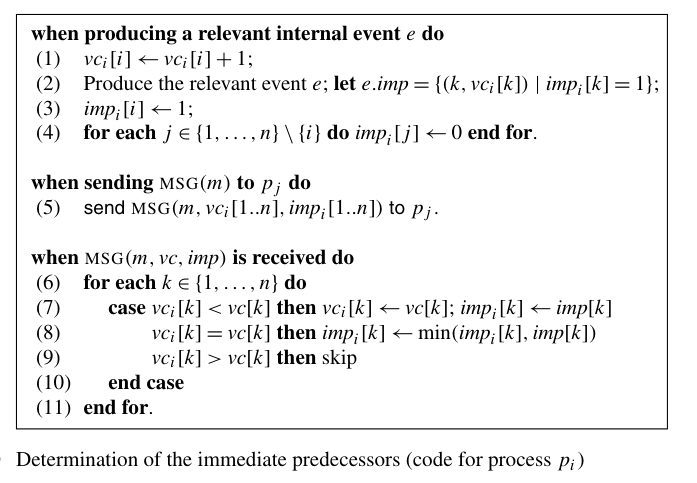
\includegraphics[scale=0.7]{Imagenes/algoIPT.png}
            \label{fig:ejemplo1}
        \end{subfigure}
    \end{figure}
\end{frame}
%%%%%%%%%%%%%%%%%%%% Especificación:
\begin{frame}[fragile]{Vector Clocks in Action:}{Immediate Precessors}
    \justifying
    \textbf{Casos para la actualización del predecesor inmediato}
    \begin{figure}
        \centering
        \begin{subfigure}[b]{\textwidth}
            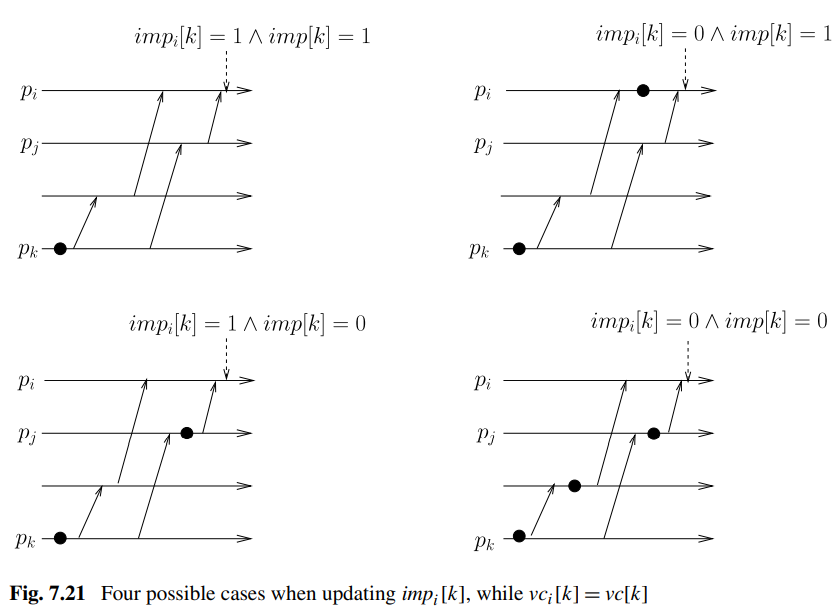
\includegraphics[scale=0.5]{Imagenes/casosActualizarIPT.png}
            \label{fig:ejemplo1}
        \end{subfigure}
    \end{figure}
\end{frame}
%----------------------------------------------------------
%\subsection{Detección de una conjunción de predicados locales estables.}
%%%%%%%%%%%%%%%%% Conjunción de predicados estables.
\begin{frame}[fragile]{Aplicación:}{Detección de conjunciones de predicados estables.}
  \justifying
  \textbf{Def.} Un predicado es local para $p_i$ \textit{\textbf{Sii}}
  se encuentra en variables de $p_i$ solamente.
  
  \textbf{Def.} El predicado $LP_i$ es estable \textit{\textbf{Sii}}
  en cuanto se vuelva verdadero, este permanece así siempre.
  
  \textbf{Notación:} $\sigma_i \models LP_i$. Indica que el estado local $\sigma_i$
  de $p_i$ satisface el predicado $LP_i$.
  
  \textbf{Def.} Sea $\{p_1, \dotsm, p_n\}$ un sistema distribuido y $LP_1, \dotsm, LP_n$ $n$
  predicados locales, uno por proceso (con su respectivo proceso). Un \textit{estado global
  consistente} $\sum = (\sigma_1, \dotsm, \sigma_n)$ satisface el predicado global
  $LP_1 \land \dotsm \land LP_n$ denotado por
  \[\sum \models \bigwedge_i LP_i\]
  siempre que $\bigwedge_i (\sigma_i \models LP_i)$.
  \setblockstyle{native} % Default behavior, optional line.
  \begin{center}
    \begin{minipage}[b]{0.5\textwidth}
      \begin{exampleblock}{Problema.}
        \justifying
        Detectemos sobre la \textit{historia} del sistema, y sin utilizar controles de mensajes
        adicionales, el primer estado global consistente $\Sigma$ que satisface una conjunción
        de predicados locales estables.
      \end{exampleblock}    
    \end{minipage}
  \end{center}
\end{frame}

%%%%%%%%%%%%%%%%% Conjunción de predicados estables. Solución.
\begin{frame}[fragile]{Aplicación:}{Solución.}
  \justifying
\begin{figure}
    \centering
    \begin{subfigure}[b]{0.5\textwidth}
        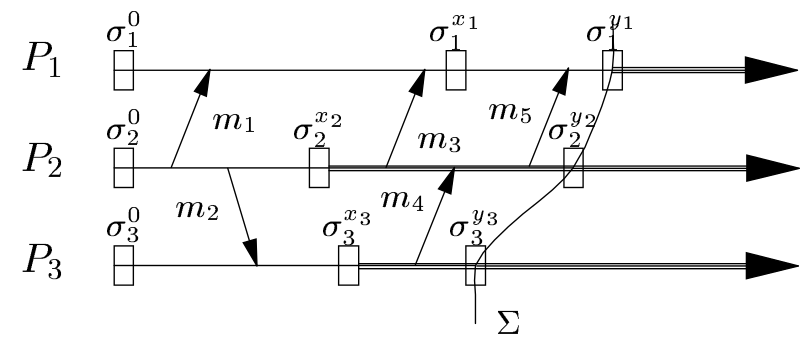
\includegraphics[width=\textwidth]{./Ejemplo1}
        \caption{Ejemplo 1.}
        \label{fig:ejemplo1}
    \end{subfigure}
    ~ %add desired spacing between images, e. g. ~, \quad, \qquad, \hfill etc. 
      %(or a blank line to force the subfigure onto a new line)
    \begin{subfigure}[b]{0.5\textwidth}
        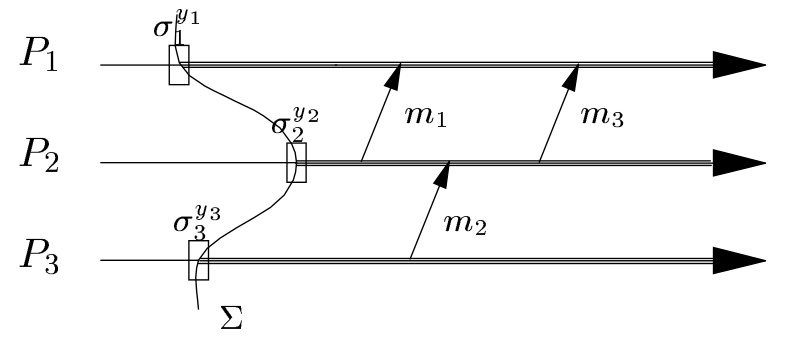
\includegraphics[width=\textwidth]{./Ejemplo2}
        \caption{Ejemplo 2.}
        \label{fig:ejemplo2}
    \end{subfigure}
    \caption{Detección de una conjunción local estable.}\label{fig:Deteccion.}
\end{figure}
\end{frame}

%\subsection{Un problema de conjuntos: Conjuntos Posibles e Imposibles.}
%%%%%%%%%%%%%%%%% Conjuntos Imposibles.
\begin{frame}[fragile]{Conjuntos Imposibles:}{Problema.}
  \justifying
  El problema de los \textit{conjuntos imposibles} establece:
  \begin{center}
    \textit{Dado un conjunto con n etiquetas vectoriales de k entradas cada una, decidir si
    es posible o no.}
  \end{center}

  \textbf{Ejemplo:}
  \begin{figure}
    \centering
    \begin{subfigure}[b]{0.3\textwidth}
      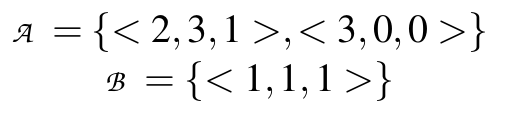
\includegraphics[width=\textwidth]{./Imagenes/Conjuntos}
        \caption{Conjuntos.}
        \label{fig:Conjuntos.}
    \end{subfigure}
    ~ %add desired spacing between images, e. g. ~, \quad, \qquad, \hfill etc. 
      %(or a blank line to force the subfigure onto a new line)
    \begin{subfigure}[b]{0.7\textwidth}
        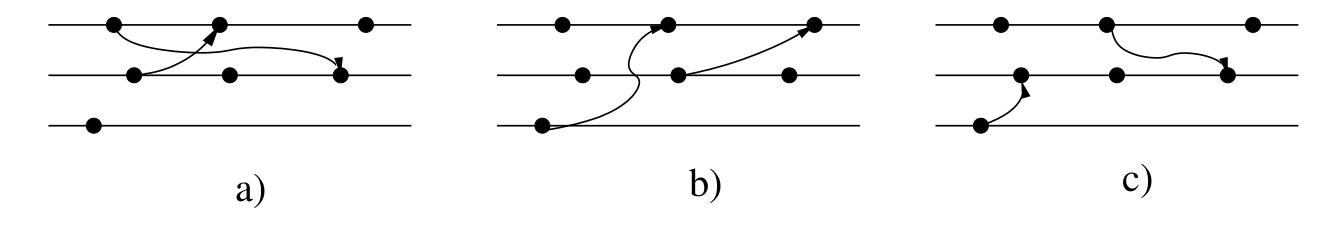
\includegraphics[width=\textwidth]{./Imagenes/Historia}
        \caption{Historias.}
        \label{fig:Historias.}
    \end{subfigure}
    \caption{Detectando conjuntos.}\label{fig:ConjuntosImposibles.}
  \end{figure}
\end{frame}


%%%%%%%%%%%%%%%%%%%%%%%%%%%%%%%%% Introducción:
\begin{frame}[plain]
  \begin{figure}
    \centering
    \begin{subfigure}[b]{0.6\textwidth}
      
\includegraphics[width=\textwidth]{./Imagenes/T3}
    \end{subfigure}
  \end{figure}
\end{frame}

%%%%%%%%%%%%%% Bloom: extra.
%\section{Relojes de Bloom.}
%\subsection{Filtro Bloom.}
%%%%%%%%%%%%%%%%% Relojes Bloom.
\begin{frame}[fragile]{Relojes Bloom:}{Filtro Bloom.}
  \justifying
  \textbf{Def.} El \textit{filtro Bloom} es una estructura de datos,
  probabilística, eficiente en espacio diseñada para verificar rápidamente
  si un elemento esta contenido en conjunto.\newline

  \textbf{Algoritmo.}
  \begin{enumerate}
  \item Definir $k$ funciones \textit{HASH} independientes.
  \item Definir un arreglo de \code{bits} con $m$ \code{bits},
    todos inicialmente igual a $0$.
  \item Para agregar un elemento al \textit{filtro bloom}, hacer
    \begin{enumerate}
    \item Pasamos el elemento, digamos $x$, por las $k$ \textit{funciones
      hash}.
    \item Cada hash apunta a un índice en el arreglo de \code{bits}
    \item La posición a la que se apunte cambia de $0$ a $1$.
    \end{enumerate}
  \end{enumerate}

  \begin{figure}
    \centering
    \begin{subfigure}[b]{0.5\textwidth}
      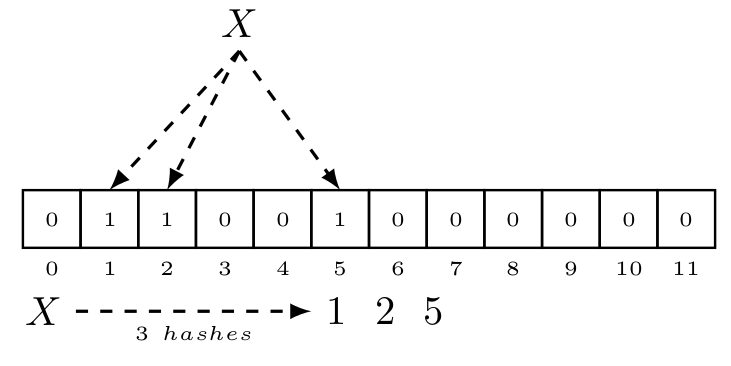
\includegraphics[width=\textwidth]{./Imagenes/Hash01}
      \caption{Inserción al filtro.}
      \label{fig:Ejemplo de Hash(X).}
    \end{subfigure}
  \end{figure}
\end{frame}

%%%%%%%%%%%%%%%%% Relojes Bloom.
\begin{frame}[fragile]{Relojes Bloom:}{Filtro Bloom. Falsos positivos.}
  \justifying
  ¿Será cierto qué todos los elementos para los cuales
  las \textit{hash-funciones} nos regresen valores que en
  el \textit{bloom-filtro}  tienen asigando $1$,
  son valores que han sido introducidos al filtro?
  \begin{figure}
    \centering
    \begin{subfigure}[b]{0.5\textwidth}
      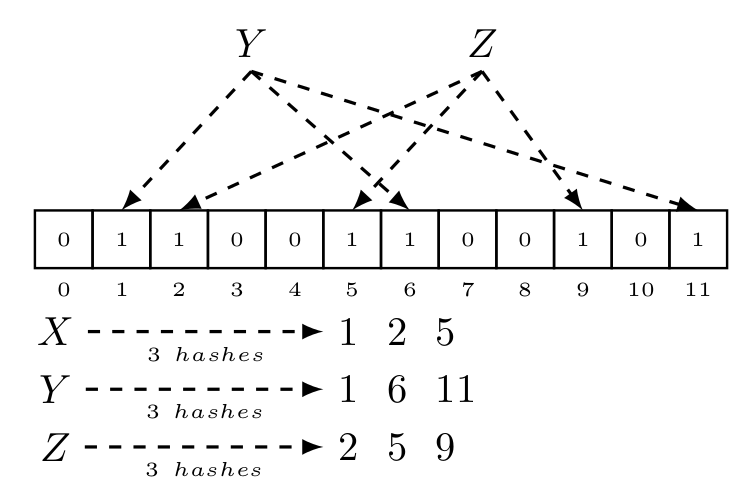
\includegraphics[width=\textwidth]{./Imagenes/FalsosPositivos}
      \caption{Falsos Positivos.}
      \label{fig:Ejemplo de un Falso Positivo.}
    \end{subfigure}
  \end{figure}
  ¿Qué podemos hacer? ...
\end{frame}


%%%%%%%%%%%%%%%%% Relojes Bloom.
\begin{frame}[fragile]{Relojes Bloom:}{Filtro Bloom. Mejoras.}
  \justifying
  ¿Qué podemos hacer? ...\newline
  Podemos controlar la tasa de falsos positivos ajustando:
  \begin{enumerate}
  \item El tamaño del \textit{bloom-filtro} ($m$).
  \item El número de elementos insertados en el filtro ($n$).
  \item El número de \textit{hash-funciones} ($k$) utilizadas en la codificación.
  \end{enumerate}
  y por medio de la ecuación:
  \[\left(1 - \left(1 - \frac{1}{m}\right)^{kn}\right)^k\]
  \textbf{Idea Intuitiva:}
  \begin{itemize}
  \item $1 - \frac{1}{m}$ es la probabilidad de tener un \code{bit} en
    el filtro que no este establecido como $1$ por alguna determinada
    función.
  \item $\left(1 - \frac{1}{m}\right)^k$ es la probabilidad de que un bit
    en particular no se establezca en uno, dado que $k$ hashes pueden
    señalarlo potencialmente.
  \item $\left(1 - \frac{1}{m}\right)^{kn}$ es la probabilidad de que un
    bit en particular siga siendo cero después de $n$ elementos.
  \item $\left(1 - \left(1 - \frac{1}{m}\right)^{kn}\right)^k$ es la probabilidad
    de que $k$ índices sean $1$ después de insertar n elementos, también
    conocido como tasa de falsos positivos.
  \end{itemize}
\end{frame}

%\subsection{Algoritmo.}
%%%%%%%%%%%%%%%%% Relojes Bloom.
\begin{frame}[fragile]{Relojes Bloom:}{Filtro Bloom. Mejoras.}
  \justifying
  ¿Qué podemos hacer? ...\newline
  Podemos usar una variante de \textit{bloom-filtros} con conteo
  de entradas, como se muestra en el siguiente ejemplo:
    \begin{figure}
    \centering
    \begin{subfigure}[b]{0.5\textwidth}
      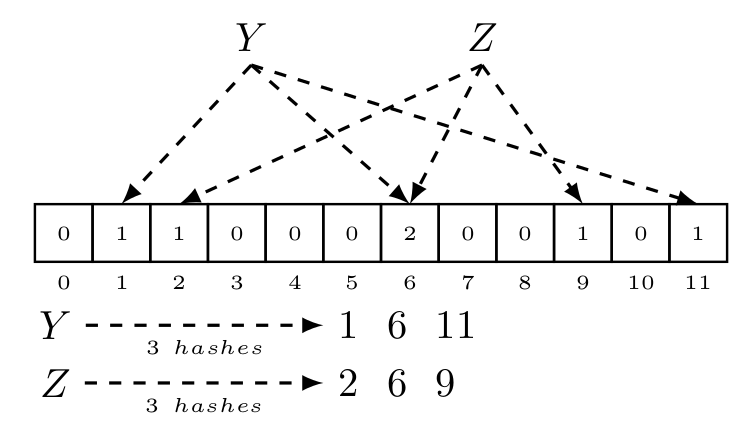
\includegraphics[width=\textwidth]{./Imagenes/CountingBloomClock}
      \caption{Filtro de Bloom tipo contador.}
      \label{fig:Ejemplo de un CountingBloomClock.}
    \end{subfigure}
  \end{figure}
\end{frame}

%%%%%%%%%%%%%%%%% Relojes Bloom.
\begin{frame}[fragile]{Relojes Bloom:}{Algoritmo.}
  \justifying
  A continuación se describe el algoritmo usado en la
  dispersión de tiempos:
  \begin{enumerate}
  \item Definimos el tamaño del \textit{bloom-filtro-conteo}
    $m$ y las $k$ \textit{hash-funciones}.
  \item Cada vez que un nodo tiene un evento interno, procesa ese evento
    con $k$ \textit{hash-funciones} e incrementa su filtro. Luego envía
    ese filtro de floración a todos los demás nodos.
  \item Cada vez que un nodo recibe un evento, actualiza su filtro
    tomando el valor máximo de su filtro y el filtro receptor.
  \end{enumerate}
  \textbf{Ejemplo:}
      \begin{figure}
    \centering
    \begin{subfigure}[b]{0.45\textwidth}
      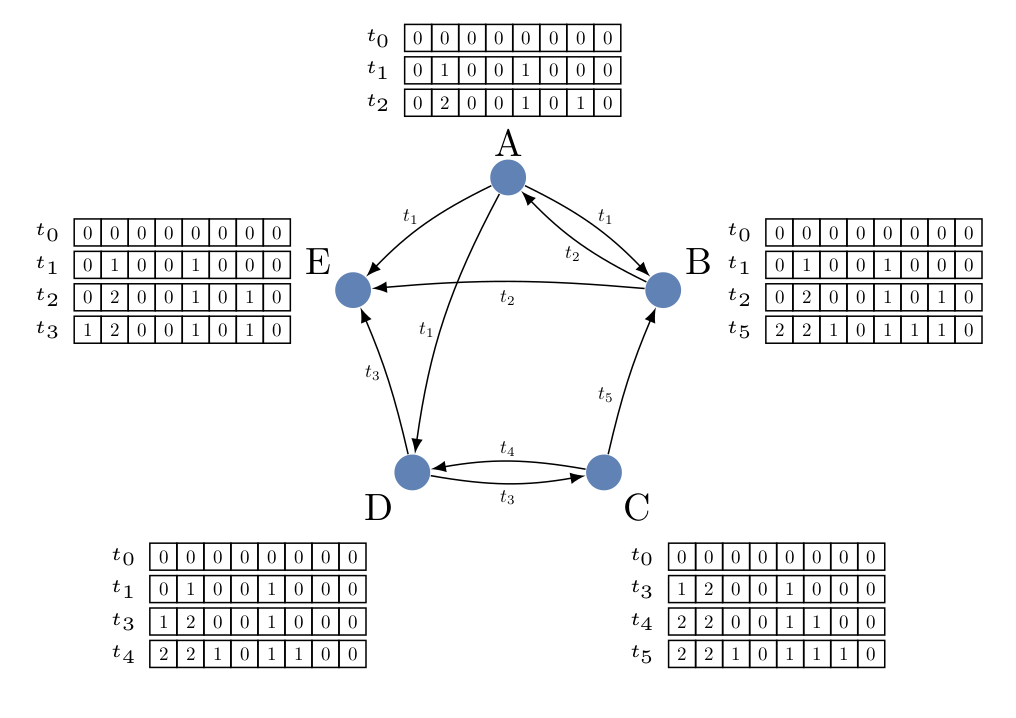
\includegraphics[width=\textwidth]{./Imagenes/RelojBloom}
      \caption{Reloj de Bloom.}
      \label{fig:Ejemplo de un CountingBloomClock.}
    \end{subfigure}
  \end{figure}
\end{frame}

\begin{frame}[fragile]{Relojes Bloom:}{Ejecución.}
  \justifying
  \textbf{Ejemplo:}
      \begin{figure}
    \centering
    \begin{subfigure}[b]{0.8\textwidth}
      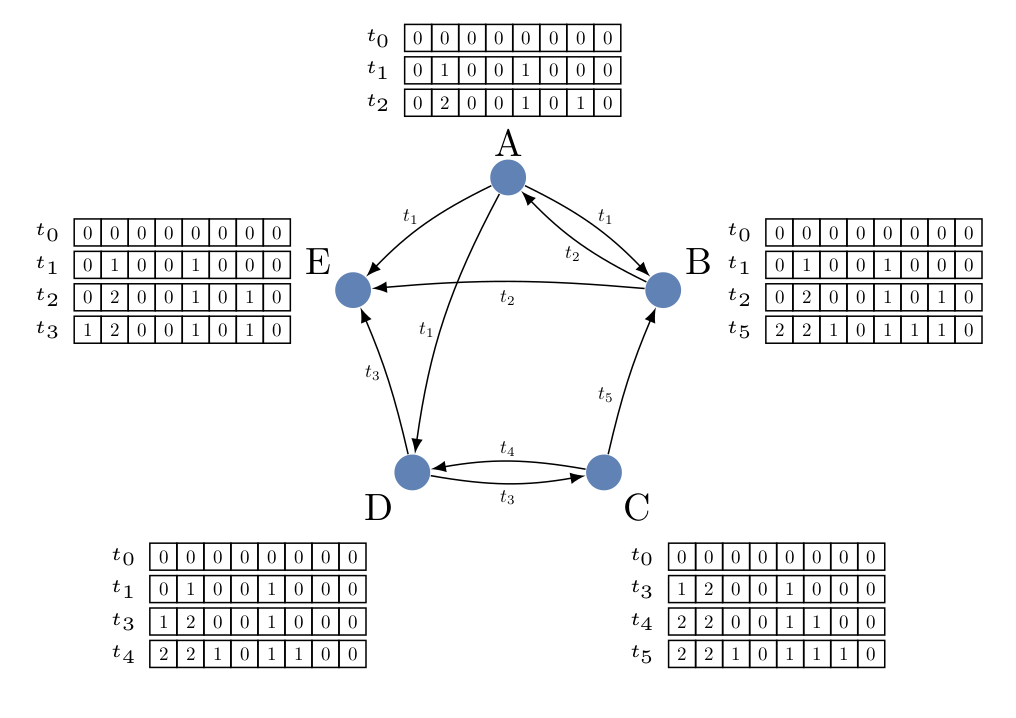
\includegraphics[width=\textwidth]{./Imagenes/RelojBloom}
      \caption{Reloj de Bloom.}
      \label{fig:Ejemplo de un CountingBloomClock.}
    \end{subfigure}
  \end{figure}
\end{frame}

%%%%%%%%%%%%%%%%%%%%%%%%%%%%% Ya se terminó!!
\begin{frame}[fragile]{Queremos 10.}{¡Muchas gracias!}
  \center {\Huge¡¡$\mathbb{AL\ FIN!!}$}
  
  \begin{figure}
    \centering
    \begin{subfigure}[b]{0.4\textwidth}
      
\includegraphics[width=\textwidth]{./Imagenes/Agradecimientos}
    \end{subfigure}
    ~ %add desired spacing between images, e. g. ~, \quad, \qquad, \hfill etc. 
      %(or a blank line to force the subfigure onto a new line)
    \begin{subfigure}[b]{0.3\textwidth}
        
\includegraphics[width=\textwidth]{./Imagenes/Fin}
    \end{subfigure}
    \end{figure}
\end{frame}

\end{document}
